\section{Experimental validation}\label{sec:experiments}

\todo[inline]{WIP}

In this section, we aim to validate the utility of the CLEAVE framework through a series of experiments.
In particular, we wish to show the utility of CLEAVE as a tool for repeatable and scalable benchmarking of \acp{NCS} in Edge environments.

\todo[inline]{talk about goal of experiments}

This section is structured in two parts.
\Cref{ssec:expsetup} details the experimental setup and describes the experiments performed.
\Cref{ssec:results} then presents and discusses the numerical results.

\subsection{Experimental Setup}\label{ssec:expsetup}

The \acl{NCS} employed for these experiments corresponds to an inverted pendulum, chosen for to its relative simplicity as well as prevalence in the field of automatic control as one of the fundamental examples of linear control.
The physical system, represented in \cref{fig:invpend}, is implemented as a real-time discrete-time physical emulation using CLEAVE's API and a 2D physics library~\autocite{chipmunk2d,pymunk}, executed at a constant \SI{120}{\hertz}.
For the controller, a proportional-differential strategy is employed, implemented using the framework Controller API and the NumPy numeric computation library~\autocite{harris2020array}.

\begin{figure}
    \centering
    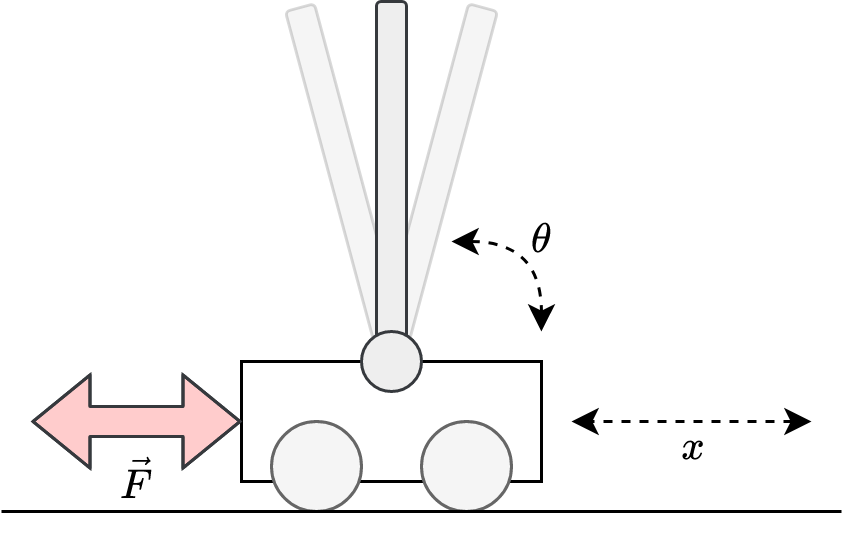
\includegraphics[width=.95\columnwidth]{images/inverted_pendulum.png}
    \caption{
        The two-dimensional inverted pendulum system.
        The cart moves on the X-axis, and the pendulum on top of it swings freely.
        The objective of the system is to balance the pendulum vertically through the application of horizontal forces on the cart.
    }\label{fig:invpend}
\end{figure}

We depict our experimental setup in \cref{fig:cleave:expsetup}, consisting of a single control loop deployed across a pair of consumer-grade computing devices.
We employ a Raspberry Pi 4B single-board computer together with a general-purpose \verb|x86_64|-based workstation; the \ac{OS} configured on both corresponds to Ubuntu Server 20.04 LTS~\cite{Ubuntu}.
These devices are connected to each other by an 802.11n WiFi link.
For ease of orchestration and re-parametrization, as well as to mimic real-world deployments, we package our CLEAVE control loop as a pair of Docker~\cite{merkel2014docker} containers.
For our main set of experiments, a two-node Docker \emph{Swarm}~\cite{Swarm2021} is set up with the \verb|x86_64| host configured as a Manager and the Raspberry Pi as a Worker node.
The containers are deployed inside the Swarm, with one of them configured as a Controller, assigned to the \verb|x86_64| host, and the other one as the Inverted Pendulum Plant and assigned to the Raspberry Pi.
These instances communicate over an overlay network which sits on top of and abstracts away the real network configuration.
Additionally, to obtain baseline results without the stochastic effects of the network, we employ a secondary ``local-only'' setup, in which we simply execute both Plant and Controller containers co-located on the \verb|x86_64| host.

\begin{figure}
    \centering
    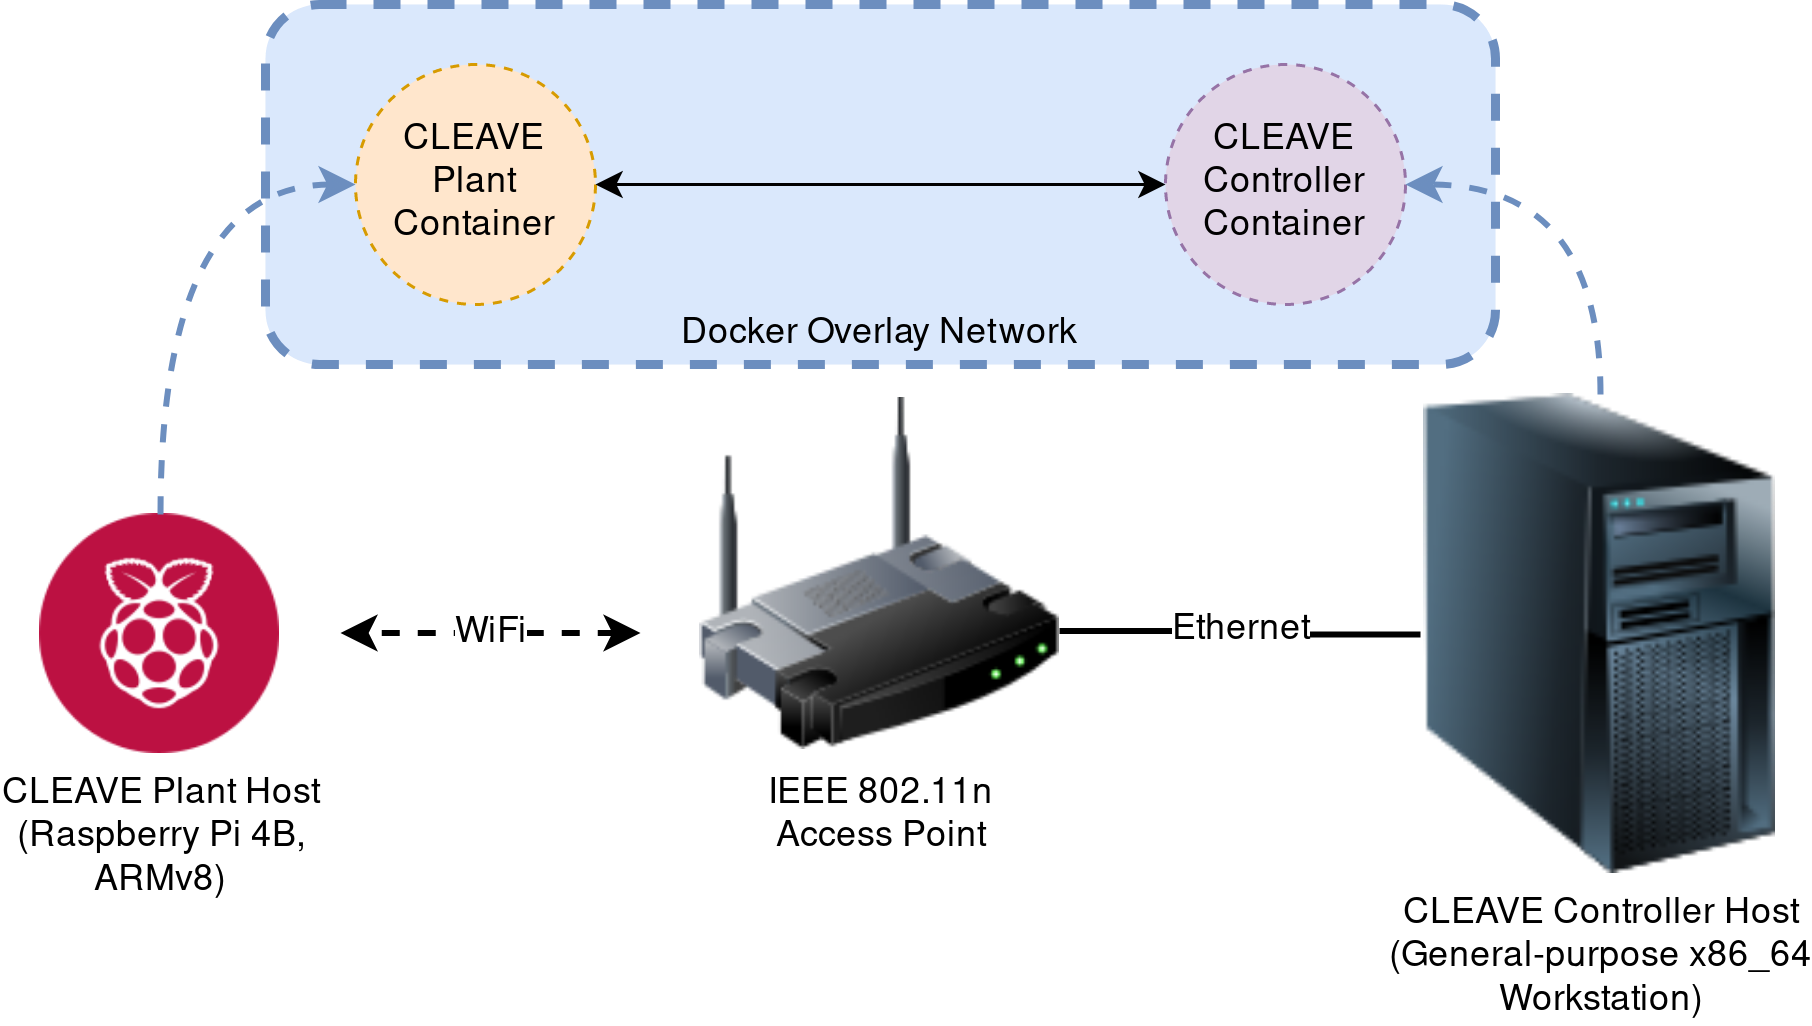
\includegraphics[width=.95\columnwidth]{images/CLEAVE_experiment_setup}
    \caption{Experimental setup. Containerized versions of the core CLEAVE emulation components are deployed inside a Docker Swarm Overlay Network spanning a Raspberry Pi 4B Plant host connected to an x86 Controller host over a 802.11n WiFi link.}\label{fig:cleave:expsetup}
\end{figure}

These setups are then used to run a series of experiments with varying parametrization of the controlled system.
Specifically, we modify:
\begin{itemize}
    \item the sampling rate of the Plant state, setting it to \SIlist[list-units=single,list-final-separator={, or }]{5;10;20;40;60}{\hertz};
    \item the responsiveness of the Controller, by adding fixed delays of  \SIlist[list-units=single,list-final-separator={, or }]{0;25;50;100}{\milli\second} after the processing of each sample.
\end{itemize}
We repeat each combination of these parameters at least \num{10} times, for both the networked and ``local-only'' setups; experiments with interesting and relevant results are then repeated an additional \num{20} times for better statistical significance in the results.
During each repetition, we collect detailed data on both the state of the controlled system as well as on the data sent over the network.

\subsection{Results}\label{ssec:results}